\chapter{Introduction}
\label{ch:intro}

\section{Motivation}
\label{sec:motivation}

Automated assembly is widely used where products have to be manufactured with high repeatability, consistent quality, and limited manual intervention. However, many assembly tasks are not only defined by moving a part from one pose to another. They involve physical contact between components, where small geometric deviations can decide whether the task succeeds, requires correction, or fails. Robotic insertion is a typical example of such a contact-rich assembly process. A peg, rod, or component has to be guided into a corresponding opening, but even small errors in position, orientation, tolerance, or peg-and-hole geometry can lead to sliding, wedging, jamming, or force-limit failures \cite{xuCompareContactModelbased2019,tangAutonomousAlignmentPeg2016,feiContactJammingAnalysis2004b}.

This makes robotic insertion difficult to analyze from the nominal task geometry alone. The same programmed motion can lead to different outcomes depending on the exact start pose, the angular alignment of the inserted part, the available clearance, the gripper condition, and the force settings used during insertion. At the same time, these physical effects are reflected in the signals recorded by the robot. Force and torque measurements, robot pose, joint motion, and actuator-related signals describe how the insertion evolves over time and can therefore contain information about whether an insertion is successful and in combination with metadata why it fails.

For this reason, robotic insertion is not only a control problem, but also a dataset problem. A useful dataset should not only contain successful and failed insertion attempts, but also describe under which physical and experimental conditions these attempts were recorded. If the dataset is linked to structured metadata, it becomes possible to form specific subgroups of samples and analyze them separately. Such subgroups can represent, for example, different geometries, tolerance levels, gripper configurations, recorded batches, position offsets, tilt levels, or force settings. This makes the dataset queryable with respect to its exact physical insertion properties, instead of treating it as one uniform collection of time series.

The motivation of this thesis is therefore to create and analyze a structured robotic insertion dataset that connects multivariate robot time series with detailed metadata. The dataset is used to investigate the central research question of this thesis:

\begin{quote}
\textbf{How can a structured robotic insertion dataset with multivariate robot time-series data and metadata be used to identify which insertion conditions have an impact on the physical insertion success rates, which insertion conditions have an impact on classification performance, and where these two perspectives overlap and differ?}
\end{quote}

\section{Research Approach}
\label{sec:research_approach}

\begin{figure}[htbp]
    \centering
    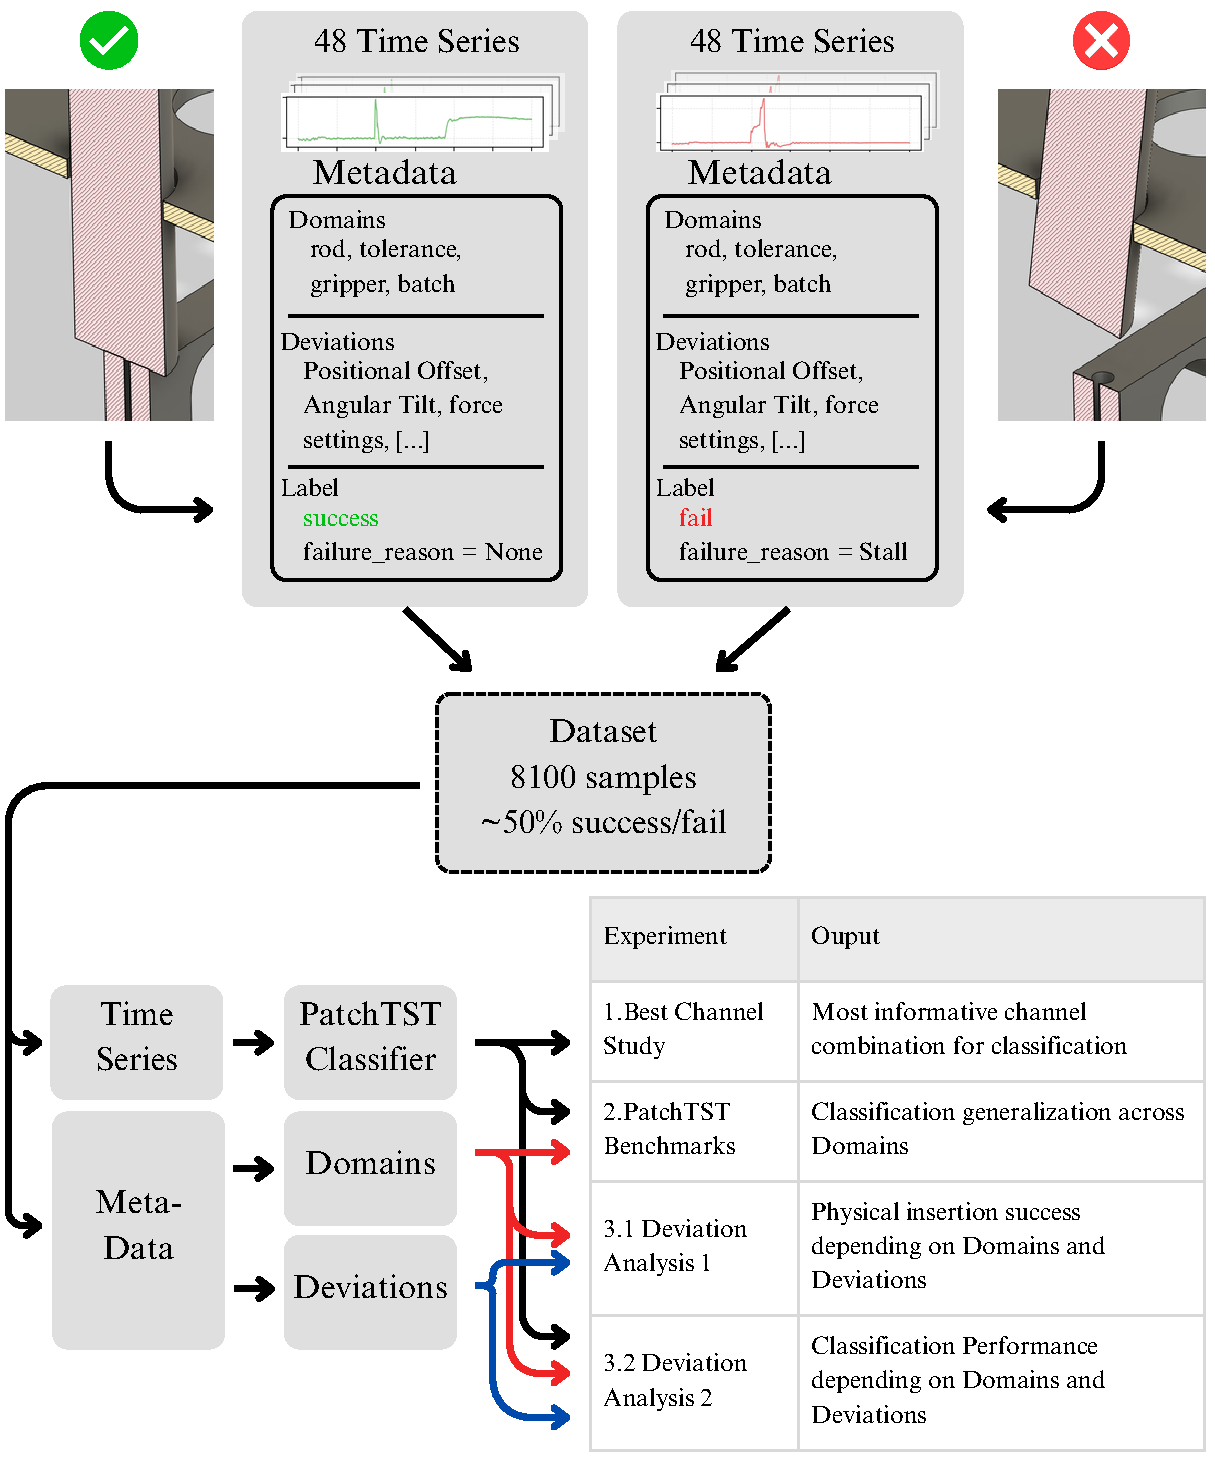
\includegraphics[width=0.97\linewidth]{chapters/1-introduction/thesis_overview.pdf}
    \caption{Overview of the research approach, from robotic insertion attempts to structured dataset analysis and practical conclusions.}
    \label{fig:intro_research_approach}
\end{figure}

The research approach of this thesis is summarized in \figref{fig:intro_research_approach}. The starting point is a robotic insertion setup in which a UR5e robot performs repeated peg-in-hole insertion attempts under systematically varied insertion conditions. Each attempt results either in a successful insertion (top left CAD section view in \figref{fig:intro_research_approach}) or in a failed insertion (top right CAD section view in \figref{fig:intro_research_approach}) caused by effects such as misalignment, stalling/jamming, force-limit termination, or timeout.

Each insertion attempt is stored as one dataset sample. A sample consists of a multivariate robot time series with 48 channels recorded direclty from the robots sensors and metadata containing the binary success label, the failure reason (if present), and the physical and experimental conditions of the attempt, categorized in domains and deviations. A domain is the general term describing the used rod type, tolerance level, gripper configuration and recording batch from one insertion. A deviation describes among others the applied position offset, applied tilt, force level, force limit. The combination of time-series data and metadata is central to the thesis, because it makes the dataset queryable. Instead of evaluating only one global classification result, a specific subset can be selected and analyzed separately.

PatchTST is used as the main classification model in this thesis. As shown conceptually in \figref{fig:intro_research_approach}, the classifier receives the recorded time-series data, trains on a specific subset, specified by the used experiment, and predicts whether an insertion attempt was successful or failed. Internally, PatchTST transforms the time series into fixed-length patches, embeds these patches as tokens, and processes them with a Transformer-based architecture. For the binary insertion task, the model produces a single output logit, which is converted into a success probability and classified using a decision threshold.

To answer the research question four connected experiments are conducted. First, the best channel study evaluates which subset of the 48 robot signals are most useful for insertion-success classification. This determines the final input configuration used for the following experiments. Second, the benchmark experiments evaluate how classification performance changes under different train-test splits, from an in-distribution split to increasingly difficult unseen-condition splits. Third, Deviation Analysis I uses the metadata directly to determine which insertion conditions impact the physical success rate. Fourth, Deviation Analysis II combines the metadata with the classifier predictions to determine which conditions are difficult for the model and where model confusion occurs.

This structure connects the physical insertion process, the dataset representation, and the classification results. The purpose is therefore not only to train a classifier with high global performance, but to use the classifier and the metadata together to analyze the dataset. This makes it possible to compare physical insertion difficulty with classification difficulty and to identify where these two perspectives overlap or differ.


% In this thesis, an \textit{insertion condition} refers to a metadata-defined subset of the dataset, such as a specific geometry--tolerance combination, gripper configuration, recording batch, position offset, tilt level, or force setting. The research question is therefore not limited to global classification accuracy. Instead, it asks how the dataset can be analyzed locally to understand both the physical behavior of the insertion process and the behavior of a machine-learning classifier.

\section{Main Findings}
\label{sec}

The central research question is answered by showing that the recorded robotic insertion dataset enables insertion difficulty to be analyzed from the perspective of physical insertion success through metadata and classification performance through time-series classification. The results show that physical insertion succes and classification performance often overlap in specific cases, but differ in others.

First, force/torque signals provide the strongest individual signal group, but the best classification results are achieved when force/torque is combined with TCP pose, joint velocity, and current consumption using a PatchTST model variant with higher capacity. This indicates that insertion success is not represented by one signal modality alone, but by diverse information about contact interaction, robot state, motion dynamics, and actuator load. The benchmark experiments further show that classification is strongest under in-distribution conditions, where samples for the test set are randomly assigned, and that classification remains possible under several unseen-domain splits, with the strongest generalization performance being to unseen tolerance levels. However, rectangular geometries and recording-batch-level shifts are substantially more difficult to classify, showing that the dataset contains both generalizable patterns and real classification challenges.

Second, the metadata-based analysis identifies which deviations are physically difficult for the insertion process. The most impactful global influence on physical success is angular misalignment (tilt). Increasing tilt reduces the success rate more clearly than the tested position offsets. The force interaction is another important factor and is defined as a combination of commanded insertion force level and force limit using to detect failures. Because the force level and force limit cannot be interpreted independently, a small or negative difference between force limit and force level strongly reduces the physical success rate and changes the dominant failure causes. In addition, local metadata analysis can reveal setup-specific effects, such as directional asymmetries that indicate a possible bias of the nominal insertion pose.

Third, Deviation Analysis II: Model Confusion shows that physical low insertion success rates are not necessarily difficult to classify. Large tilt reduces the physical success rate, but often produces signal patterns that are information-rich for the classifier. In contrast, some force-interaction groups are more problematic because they create locally imbalanced or ambiguous signal patterns. The analysis shows that a physically undesirable success rate close to 50\% can be useful for classification, because both successful and failed insertions are sufficiently represented. Conversely, physical high insertion success rates or very low success rates can be problematic for the classifier because they make local classes heavily imbalance, which causes the underrepresented class to be misclassified.

Overall, the main finding is that the dataset itself is the central result of the thesis. It does not only enable insertion-success classification, but also allows the relationship between physical insertion variation and classification behavior to be analyzed. The combination of multivariate time-series data, domain and deviation specific metadata, and model predictions makes it possible to identify which insertion conditions are impactful to physical insertion success, which insertion conditions are difficult to classify, and where these two perspectives overlap and differ.


\section{Thesis Structure}
\label{sec:thesis_structure}

This thesis is structured as follows. 

Chapter \ref{ch:intro} introduces the motivation, research question, research approach, and main findings of the thesis.

Chapter \ref{ch:state-of-the-art} presents the background and related work on robotic insertion, time-series classification, and relevant machine-learning methods.

Chapter \ref{ch:rob_setup} describes the robotic system and experimental setup used for data collection.

Chapter \ref{ch:dataset} explains the dataset construction, labeling procedure, metadata structure, and preprocessing steps.

Chapter \ref{ch:methodology} introduces the PatchTST-based time-series classification pipeline, including the model adaptation, training procedure, and evaluation metrics.

Chapter \ref{ch:experiments} defines the conducted experiments. This includes the best channel study, the benchmark experiments, and the two deviation analyses.

Chapter \ref{ch:results} presents and discusses the results of these experiments, with focus on classification performance, generalization behavior, physical insertion success, and model confusion.

Chapter \ref{ch:conclusion} concludes the thesis by answering the research question, deriving practical recommendations for insertion setup design, and discussing limitations and future work.

The appendix contains additional results for the Benchmark 3 test-loss evaluation.

